\clearpage
\section{Automatyzacja pracy z submodułami (JC)}
\label{sec:gitio}

Ninejszy rozdział jest poświęcony obsłudze wielopoziomowej struktury opartej o \emph{git submodules} obecnej w projekcie GGSS. Przedstawione zostaną plusy oraz minusy zastosowanego w trakcie pracy inżynierskiej rozwiązania. Omówiona zostanie przygotowana przez autorów infrastruktura mająca na celu ułatwienie pracy z submodułami. Dodatkowo krótko zostanie opisane przygotowane \emph{how-to} oraz praktyki które powinno się stosować pracując z taką architekturą.

\subsection{Wprowadzenie do problematyki}

W trakcie pracy inżynierskiej, a konkretnie migracji całego projektu GGSS do systemu kontroli wersji \emph{git} zdecydowano się na wykorzystanie technologii \emph{git submodules}. Ze względu na nacisk na zwiększenie modularyzacji projektu technologia ta idealnie wpasowywała się w docelową architekurę. Zasada działania submodułów jest bardzo zbliżona do dowiązań symbolicznych stosowanych między innymi w systemach UNIX. Zamiast wskazywać na ścieżkę do folderu na lokalnym systemie submoduł wskazuje na ścieżkę do konkretnej wersji repozytorium na zewnętrznym serwerze od którego zależy nasz moduł. Rysunek \ref{fig:submodules_links} przedstawia zasadę działania submodułów oraz wpływ wersjonowania na tenże mechanizm. Wykorzystanie submodułów pozwala na w pełni odseparowaną pracę nad wybranym komponentem systemu. Nie potrzebujemy pobierać żadnych dodatkowych plików, czy też zależności w celu zmienienia kodu źródłowego. Rozwiązanie to pozwala też na skorzystanie z bardzo szybkiej inicjalizacji całego projektu jedną komendą, co zostało przedstawione w listingu \ref{lst:initialize}.

\begin{figure}[H]
    \centering
    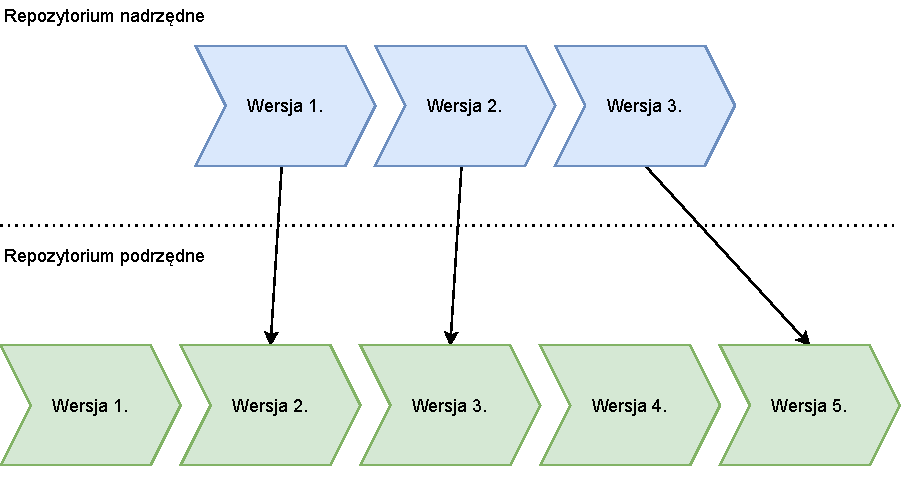
\includegraphics[width=0.9\textwidth]{submodule_links.pdf}
    \caption{Zasada działania submodułów.}
    \label{fig:submodules_links}
\end{figure}

\begin{lstlisting}[language=c++, caption={Inicjalizacja pełnej sturktury projektu jedną komendą.}, label={lst:initialize}]
root@host:/# git clone ssh://git@gitlab.cern.ch:7999/atlas-trt-dcs-ggss/ggss-all.git && cd ggss-all && git submodule update --init --recursive
Cloning into '/CERN/ggss-all/ggss-dim-cs'...
Cloning into '/CERN/ggss-all/ggss-driver'...
Cloning into '/CERN/ggss-all/ggss-oper'...
Cloning into '/CERN/ggss-all/ggss-runner'...
Cloning into '/CERN/ggss-all/ggss-spector'...
Cloning into '/CERN/ggss-all/mca-n957'...
Cloning into '/CERN/ggss-all/ggss-dim-cs/external-dim-lib'...
Cloning into '/CERN/ggss-all/ggss-dim-cs/ggss-misc'...
Cloning into '/CERN/ggss-all/ggss-driver/external-n957-lib'...
Cloning into '/CERN/ggss-all/ggss-driver/ggss-misc'...
...(13 lines truncated)
\end{lstlisting}


\subsection{Motywacja do wprowadzenia zmian}

Pomimo wielu aspektów \emph{git submodules}, które bardzo dobrze wpasowały się w, kreowaną przez autorów w trakcie pracy inżynierskiej, sturkturę technologia ta posiada też swoje minusy. Pierwszy znaczącym problemem napotkanym w trakcie pracy z submodułami było nietypowe zachowanie repozytoriów w trakcie ich inicjalizacji, a konkretnie automatyczne odłączanie ich od głównej gałęzi. Co więcej praca z submodułami wymaga od programisty zwiększonej czujności oraz stosowania dodatkowych zasad, ponieważ więcej jest miejsc na pomyłkę, co może doprowadzić do niepoprawnego działania wykorzystanych narzędzi. Kolejnym problemem napotkanym w trakcie pracy z submodułami jest czasochłonność niektórych operacji, w szczególności aktualizacji repozytorium na samym dole ``drzewa zależności``. Zmiana taka wymaga ręcznej aktualizacji po kolei każdego z repozytorium, aż do samej góry tejże skruktury co przedstawia rysunek \ref {fig:submodules_update}. Każda z aktualizacji przedstawiona na wyżej wymieionym rysunku, to tak na prawdę cztery lub więcej akcji do których wliczają się: aktualizacja repozytorium podrzędnego, dodanie wszystkich zmian do rejestru odpowiedzialnego za ich śledzenie, utworzenie nowej wersji repozytorium, opublikowanie nowej wersji na zewnętrznym serwerze.



\clearpage
\begin{figure}[H]
    \centering
    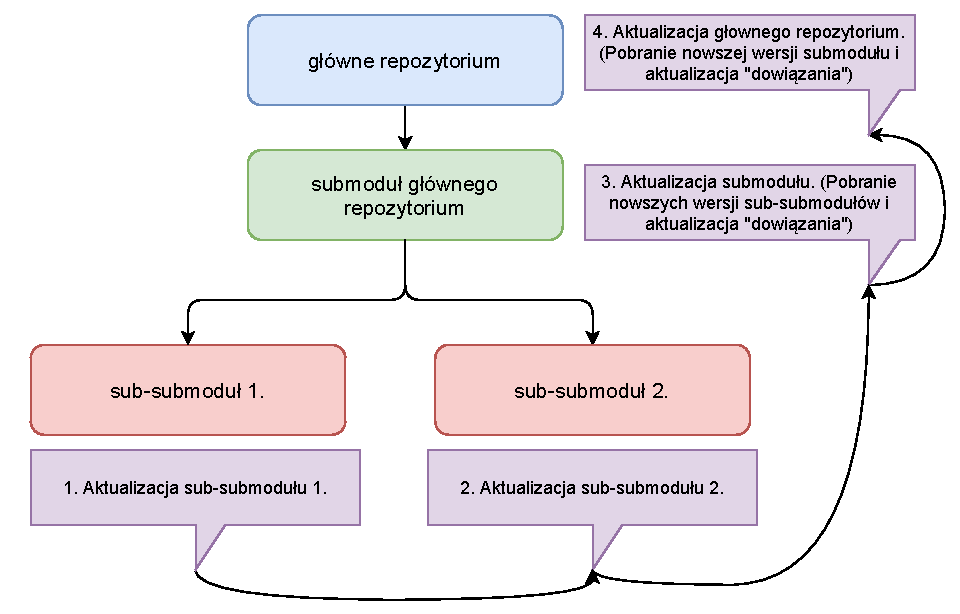
\includegraphics[width=0.9\textwidth]{submodules_update.pdf}
    \caption{Przykładowa architektura oparta o submoduły z krokami jakie należy podjąć, aby wprowadzić zmiany na ``najniższym`` poziomie.}
    \label{fig:submodules_update}
\end{figure}


\subsection{Automatyzacja z użyciem dedykowanego narzędzia}
\label{subsec:gitio}

Problemem, którego rozwiązanie pochłonęło najwięcej czasu i wymagało największego wkładu pracy przez autorów było monotonne, wielokrokowie wprowadzanie zmian do projektu, szczególnie u dołu struktury zależności. W celu rozwiązanie tego problemu przygotowano aplikacje \emph{gitio} z wykorzystaniem języka \emph{Python}. Ze względu na to, że metadane technologii \emph{git} są bardzo złożone, a opanowanie zasad węwnętrznego działania tejże technologii wymagałoby bardzo dużo czasu skorzystano z dedykowanej, do tej technologii, bilbioteki napisanej również w języku \emph{Python}.

\clearpage
Argumenty wejściowe jako przyjmuje \emph{gitio} to:
\begin{itemize}
    \item \lstinline{-h, --help} - pozwala na wyświetlnie informacji o przeznaczeniu programu oraz przyjmowanych argumentach wraz z krótkim opisem
    \item \lstinline{-p PATH, --path PATH} - ścieżka do głównego folderu zawierające drzewo repozytoriów do wyrównania
    \item \lstinline{-b BIN, --bin BIN} - ścieżka do aplikacji git. Argument ten jest wymagany jedynie, jeżeli gitio nie jest w stanie automatycznie wykryć git'a.
\end{itemize}

Przed uruchomieniem aplikacji gitio należy uprzednio przygotować repozytoria, które mają zostać poddane procesowy wyrównania. W tym celu należy wykonać następujące kroki:
\begin{itemize}
    \item sklonować główne repozytorium - \lstinline{git clone <urL>}. W celu poprawnego działania należy sklonować repozytorium z użyciem klucza ssh.
    \item zainicjalizować i zaktualizować wszystkie submoduły - \lstinline{git submodule update --init --recursive}
    \item ustawić główną gałąź na każdym z submodułów - \lstinline{git submodule foreach --recursive "git checkout master"}
\end{itemize}
Zasada działania aplikacji jest dosyć prosta, natomiast znacząco ułatwia działania z wielopoziomową strukturą opartą o \emph{git submodules}. W pierwszej kolejności gitio analizuje strukturę katalogów oraz metadane zawarte w folderach .git, dzięki czemu jest w stanie zapisać w pamięci zależności między repozytoriami. Następnie przechodząc od samego dołu drzewa zależności, czyli repozytoriów, które nie mają żadnych submodułów, wykonywane są następujące akcje:
\begin{itemize}
    \item Aktualizacja rewizji, na które wskazują submoduły do najnowszych dostępnych w zdalnym repozytorium
    \item Utworzenie nowej rewizji z zaktualizowanymi submodułami
    \item Przekazanie nowej rewizji do podłączonego zewnętrznego repozytorium.
\end{itemize}
W celach bezpieczeństwa gitio pozwala na wyrównanie wersji repozytoriów tylko na czystych repozytoriach, czyli takich, gdzie nie ma żadnych zmian od wykonania ostatniej rewizji.

Rysunek \ref{fig:gitlab_gitio} przedstawia przykładową rewizję na portalu Gitlab utworzoną z użyciem gitio. Wiadomość w ramach utworzonej rewizji, czyli "Automatic repository update", wskazuje na wykorzystanie gitio. Jedyne zmiany jakie jest w stanie wprowadzić gitio, to aktualizacja rewizji podprojektu, co widoczne również widoczne jest na wyżej wymienionym rysunku.

\begin{figure}[H]
    \centering
    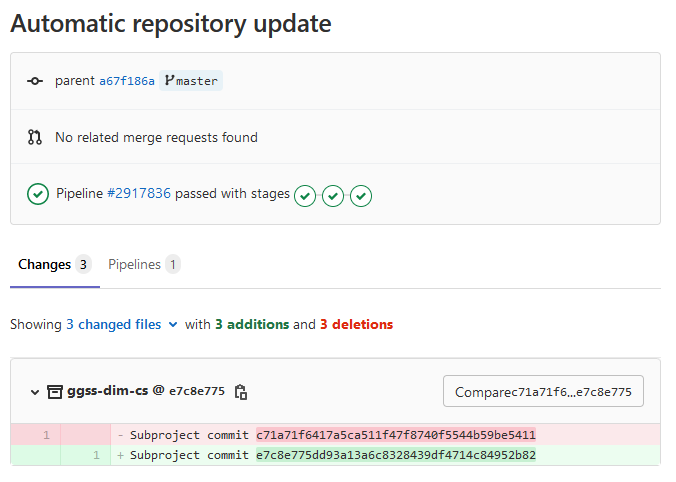
\includegraphics[width=0.9\textwidth]{gitio_gitlab.png}
    \caption{Przykładowa rewizja utworzona z użyciem gitio.}
    \label{fig:gitlab_gitio}
\end{figure}


\subsection{Dokumentacja sposobu pracy z submodułami}

Ze względu na to, że praca z repozytoriami posiadającymi submoduły wymaga dodatkowej uwagi oraz praktyk, względem pracy ze zwykłymi repozytoriami autorzy postanowili przygotować stosowaną dokumentację, która pozwala na uniknięcię poważnych błędów, które mogłyby doprowadzić do zepsucia systemu kontroli wersji.

Dokumentacja została podzielona na trzy części. Pierwsza z nich odnosi się do poprawnej inicjalizacji repozytoriów z wielopoziomowymi submodułami:
\begin{itemize}
    \item W pierwszej kolejności należy sklonować odpowiednie repozytorium z zewnętrznego serwera. W celu ułatwienia pracy z submodułami należy akcję to wykonać za pomocą protokołu ssh wraz z przypisanym odpowiednim kluczem. Oszczędzi to nam wpisywania loginu oraz hasła przy każdorazowym klonowaniu submodułów. Przykładowa komenda dla repozytorium \lstinline{ggss-all} wygląda następująco: \lstinline{git clone ssh://git@gitlab.cern.ch:7999/atlas-trt-dcs-ggss/ggss-all.git}.
    \item Po poprzednim kroku sklonowane jest jedynie główne repozytorium, brak jest zawartości folderów z submodułami. Ich inicjalizacja powinna zostać wykonana komendami \lstinline{git submodule init} oraz \lstinline{git submodule update}, natomiast w celu przyspieszenia tego procesu można wykonać jedną komendę, a mianowicie \lstinline{git submodule update --init --recursive}. Właśnie taka komenda polecana przez przez autorów do pracy z projektem ggss.
    \item Ze względu na sposób działania submodułów git przed dokonaniem zmian należy jeszcze zmienić gałęzie we wszystkich submodułach na gałąź docelową. Domyślnie inicjalizacja submodułów powoduje, że ich gałezie są w stanie oderwanym (ang. \emph{detached}), co nie pozwala na tworzenie nowych rewizji i ich publikację. W celu zbiorczego zmieniena gałęzi należy wykonać komendę \lstinline{git submodule foreach --recursive "git checkout master"}
\end{itemize}

Kolejna część dokumentacji odnosi się do porad i dobrych praktyk, które należy stosować pracując z infrastrukturą repozytoriów opartą o submoduły:
\begin{itemize}
    \item Przed rozpoczęciem pracy nad nową funkcjonalnością należy upewnić się, że korzystamy z najnowszej dostępnej wersji repozytorium oraz zależności
    \item Ze względu na użycie submodułów należy upewnić się, że ich gałąź nie jest w stanie oderwanym.
    \item Przed użyciem gitio w celu wyrównania wersji wskazywanych przez submoduły należy upewnić się, że w repozytorium nie znajdują się żadne nieopublikowane zmiany, a w przypadku ich wystąpienia należy wytworzyć i opublikowac nową rewizję recznie.
    \item Twórz nową wersję na głównej gałęzi jedynie po przetestowaniu wprowadzanych zmian.
\end{itemize}

Ostatnią cześcią dokumentacji jest króki opis słowny w jaki sposób propagować zmiany w całym projekcie ggss. Propagacja odbywa się za pomocą wyrównania wersji wskazywanych przez submoduły, a zatem przez odpowiednie skorzystanie z gitio. Więcej szczegółów jak skorzystać z gitio oraz warunków jakie należy spełnić zostały opisane w sekcji \ref{subsec:gitio}.

Niniejsza dokumentacja w wersji angielskiej dostępna jest jako plik markdown w repozytorium projektu ggss i została również dołączona do niniejszej pracy jako dodatek TUTAJ WSTAWIĆ REFERENCJE DO DODATKU.